
\section{Results}

\subsection{From PID to PH: On automatic generation of PH code of the network}
%give statistics

To simulate of the model, we generated a PINT code to be simulated by the PINT simulator\footnote{Available at \url{http://process.hitting.free.fr}}. 
For the PINT code generation we use two procedures as describe in the method section. The first procedure that detect the patterns and his code. Then the second 
procedure that generate the PINT code by taking in consideration the type of the pattern to better refine the dynamic of the system on a structural point of view.
This refinement is done by introducing the synchronization sort  which is a generalization of the cooperation sort. this allow us to avoid artificial oscillation
in the dynamic of the components of our system.
%procedure take a in parameter a pattern with its code from the procedure of detection of patterns. Afater taking 
%the pattern, the procedure will write the correct code associate to the current pattern. 
%list all the selected patterns in the biological reaction into a file. In this file, each line contains the 
%name of the nodes belonging to the current reaction and the reaction type number. The list was then parsed, line by line and, 
%after renaming the nodes using numbers (for readability and in conformity with the PINT language syntax) the corresponding PINT code
%for the PH process equivalent to each reaction was generated. This was implemented in a Java code.


\subsection{Simulation experience}
%present the simulation results
In this section we'll present the results of the simulations of the model. It will be present in two 
main sub sections. In the first, we'll present the result of simulation of model without the inclusion 
of the synchronization gate and in the second we will present result with synchronization gate. Both results
present common characteristics and show us the coherence of our approach of modelization. The common characteristics
are the following:
\begin{itemize}
 \item We can modeled large scale network in which signal goes from an input node to the output nodes.
 \item We can reproduce tendances of the dynamic of components as illustrate in \ref{rwos} and \ref{rws}.
 \item The model take in accout the stochastic and time aspect of the bihaviours of the biological system.
\end{itemize}


\subsubsection{Without the introduction of synchronization gate}
The main important remark that we can made in this result \ref{rwos} is the occurence of oscillations. This is not the expect result 
but it's coherent with the simulator properties. It's important to note that the intensity of the oscillation is link with 
the size of the concurence. Despite the presence of the oscillation, the model also reproduce the same tendances namely
the dynamic of components, the signal transduction and the taking into acount the stochastic and time aspect of the model.
\begin{figure}[!t]
\centering
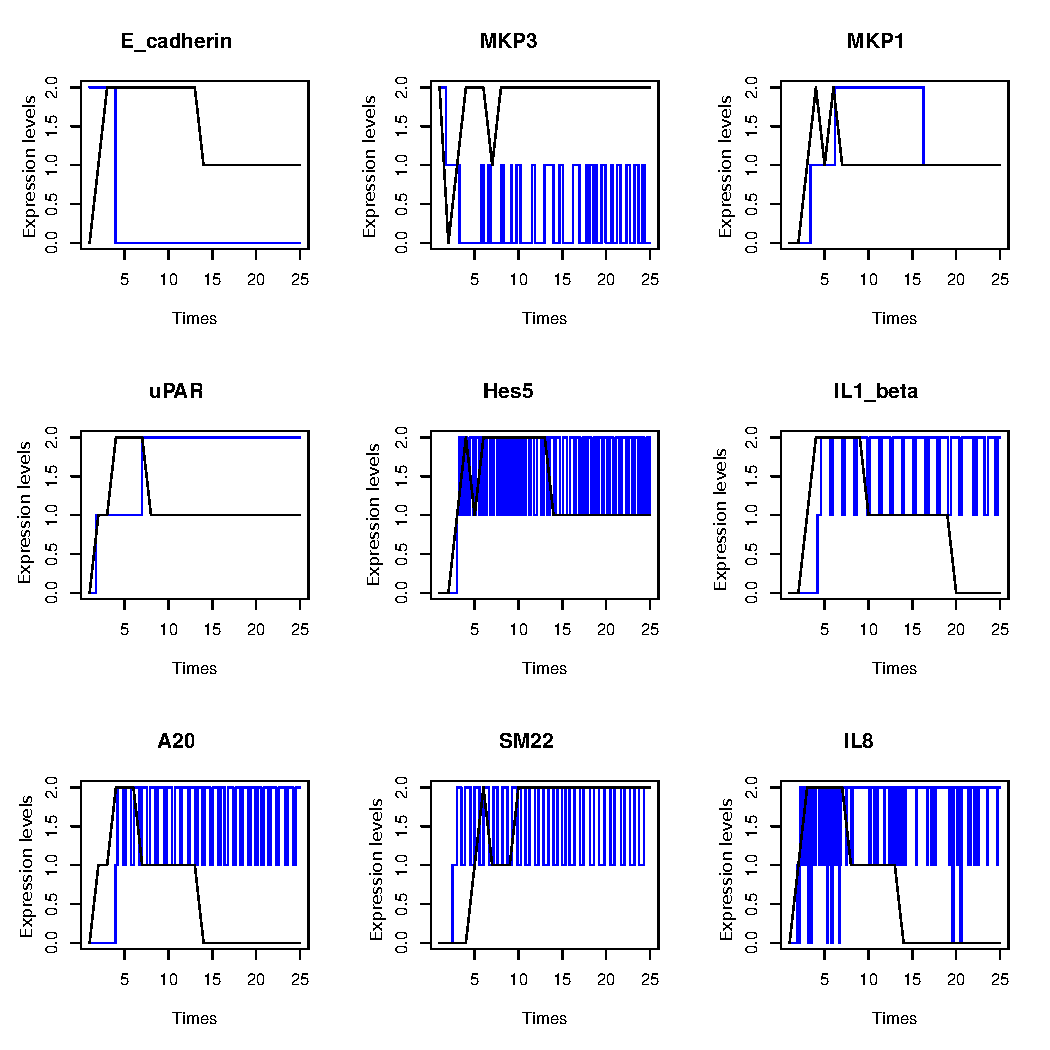
\includegraphics[width=2.5in]{images/resultWOS.pdf}
\caption{\bf Results of simulations without introducing the synchronization gate. In black line the expect behaviours
come from the discretization of time-series data. In Blue line the simulation behavior.}
\label{rwos}
\end{figure}
\subsubsection{With the introduction of synchronization gate}
On the contrary of the previous result, figure \ref{rws} show us that with the introduction of the synchronization gate, we can
reduce the impact of concurence by the introduction of the synchronization and the cooperation gates. The result show us a 
clearly elimination of the observed oscillation in figure \ref{rwos}. 

\begin{figure}[!t]
\centering
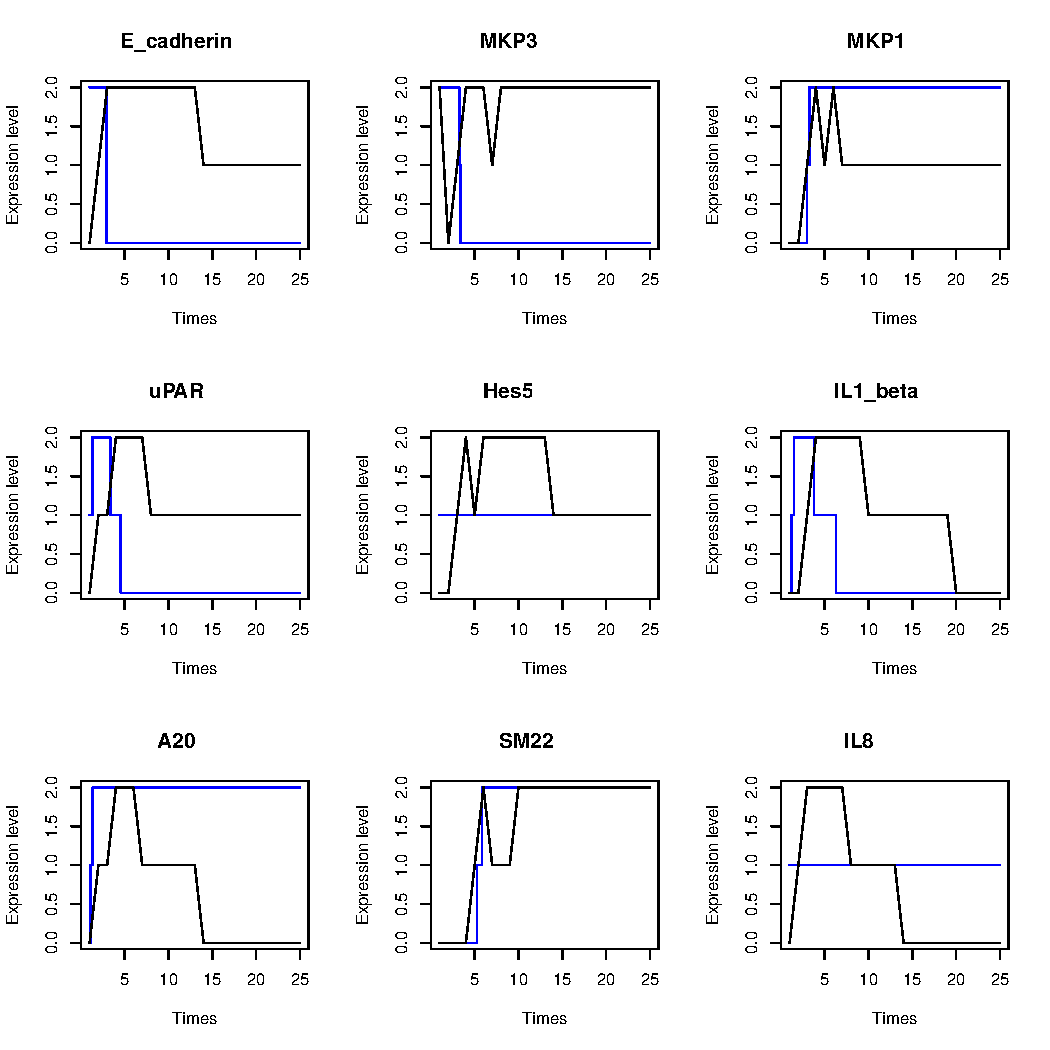
\includegraphics[width=2.5in]{images/resultWS.pdf}
\caption{\bf Results of simulation by introducing the synchronization gate. In black line the expect behaviours
come from the discretization of time-series data. In Blue line the simulation behavior.}
\label{rws}
\end{figure}


% An example of a floating figure using the graphicx package.
% Note that \label must occur AFTER (or within) \caption.
% For figures, \caption should occur after the \includegraphics.
% Note that IEEEtran v1.7 and later has special internal code that
% is designed to preserve the operation of \label within \caption
% even when the captionsoff option is in effect. However, because
% of issues like this, it may be the safest practice to put all your
% \label just after \caption rather than within \caption{}.
%
% Reminder: the "draftcls" or "draftclsnofoot", not "draft", class
% option should be used if it is desired that the figures are to be
% displayed while in draft mode.
%
%\begin{figure}[!t]
%\centering
%\includegraphics[width=2.5in]{myfigure}
% where an .eps filename suffix will be assumed under latex, 
% and a .pdf suffix will be assumed for pdflatex; or what has been declared
% via \DeclareGraphicsExtensions.
%\caption{Simulation Results}
%\label{fig_sim}
%\end{figure}

% Note that IEEE typically puts floats only at the top, even when this
% results in a large percentage of a column being occupied by floats.


% An example of a double column floating figure using two subfigures.
% (The subfig.sty package must be loaded for this to work.)
% The subfigure \label commands are set within each subfloat command, the
% \label for the overall figure must come after \caption.
% \hfil must be used as a separator to get equal spacing.
% The subfigure.sty package works much the same way, except \subfigure is
% used instead of \subfloat.
%
%\begin{figure*}[!t]
%\centerline{\subfloat[Case I]\includegraphics[width=2.5in]{subfigcase1}%
%\label{fig_first_case}}
%\hfil
%\subfloat[Case II]{\includegraphics[width=2.5in]{subfigcase2}%
%\label{fig_second_case}}}
%\caption{Simulation results}
%\label{fig_sim}
%\end{figure*}
%
% Note that often IEEE papers with subfigures do not employ subfigure
% captions (using the optional argument to \subfloat), but instead will
% reference/describe all of them (a), (b), etc., within the main caption.


% An example of a floating table. Note that, for IEEE style tables, the 
% \caption command should come BEFORE the table. Table text will default to
% \footnotesize as IEEE normally uses this smaller font for tables.
% The \label must come after \caption as always.
%
%\begin{table}[!t]
%% increase table row spacing, adjust to taste
%\renewcommand{\arraystretch}{1.3}
% if using array.sty, it might be a good idea to tweak the value of
% \extrarowheight as needed to properly center the text within the cells
%\caption{An Example of a Table}
%\label{table_example}
%\centering
%% Some packages, such as MDW tools, offer better commands for making tables
%% than the plain LaTeX2e tabular which is used here.
%\begin{tabular}{|c||c|}
%\hline
%One & Two\\
%\hline
%Three & Four\\
%\hline
%\end{tabular}
%\end{table}


% Note that IEEE does not put floats in the very first column - or typically
% anywhere on the first page for that matter. Also, in-text middle ("here")
% positioning is not used. Most IEEE journals/conferences use top floats
% exclusively. Note that, LaTeX2e, unlike IEEE journals/conferences, places
% footnotes above bottom floats. This can be corrected via the \fnbelowfloat
% command of the stfloats package.
